% !TeX root = skripta-konstitutivni-vztahy.tex
% !TeX lastmodified = 2018-11-27

\subsection{Model Bergstrőm-Boyce}\label{sec:bergstrom-boyce}
Tento model\footnote{Bergström JS, Boyce MC (1998):  Constitutive Modeling of the Large Strain Time-dependent Behavior of Elastomers, Journal of the Mechanics and Physics of Solids 45 (5), pp. 931-954.}\footnote{Bergström, J. S., Boyce, M. C. (2001): Constitutive Modeling of the Time-Dependent and Cyclic Loading of Elastomers and Application to Soft Biological Tissues, Mechanics of Materials 33, pp. 523-530.} byl navržen v~roce 1998 pro popis časově závislého chování elastomerů ve velkých deformacích.
Vychází z~modelu hyperelastického Arruda-Boyce a~rozšiřuje jej o~popis závislosti mechanické odezvy na rychlosti deformace;
tím umožňuje popsat hysterezi deformačně-napěťových křivek, stejně jako tečení a~relaxaci napětí.

Podobně jako model Arruda-Boyce vychází z~modelu prostorové sítě makromolekulárních řetězců, jejichž deformace je řízena entropickou elasticitou.
K~původní osmiřetězcové síti modelu Arruda-Boyce, popisující hyperelastickou odezvu, tedy termodynamicky rovnovážný stav, přidává druhou síť reprezentující odchylky od rovnovážného stavu.
Odpovídá to reologickému modelu Kelvin (standard linear solid), kde řetězec~A reprezentuje rovnovážnou část deformační práce a~řetězec~B nerovnovážnou část.
\begin{figure}[H]
	\centering
	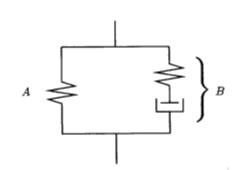
\includegraphics[height=3cm]{kelvinuv-model-ab}
	\caption{Kelvinův reologický model}
	\label{fig:kelvinuv-model-ab}
\end{figure}

\subsubsection{Dekompozice deformačního tenzoru}
Paralelní části reologického modelu mají stejnou deformaci, tedy platí
\begin{equation}
	\bm{F} = \bm{F}_A = \bm{F}_B
\end{equation}

Pro řetězec~B lze deformaci rozložit na část elastickou a neelastickou (viskózní)
\begin{equation}
	\bm{F}^B = \bm{F}^B_\text{el} \bm{F}^B_\text{vis}
\end{equation}

Na každý z~deformačních tenzorů je možné aplikovat jeho polární dekompozici (viz obr.)
\begin{figure}[H]
	\centering
	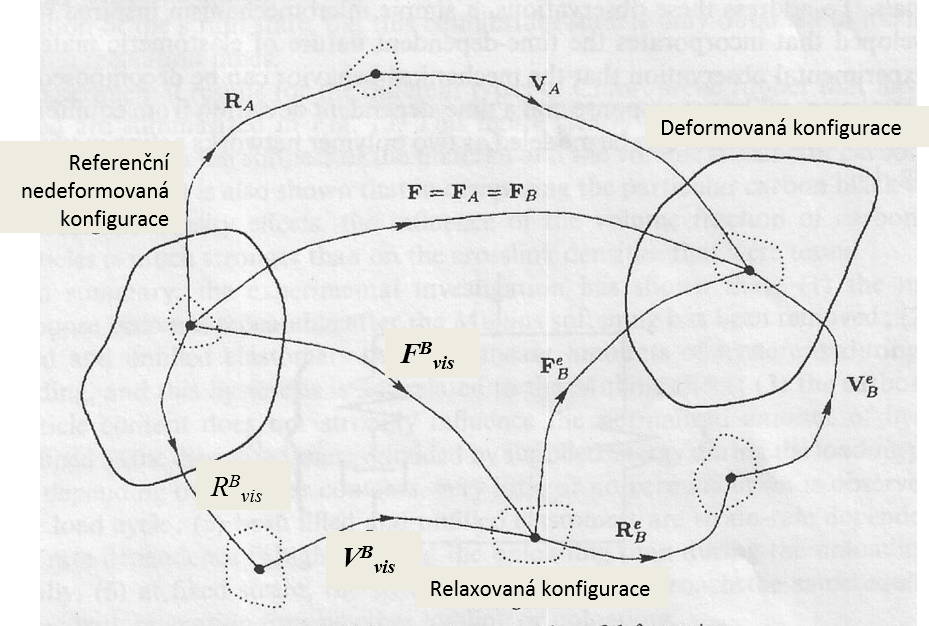
\includegraphics[width=0.7\linewidth]{polarni-dekompozice}
	\caption{Polární dekompozice}
	\label{fig:polarni-dekompozice}
\end{figure}

\subsubsection{Princip relaxace modelu Bergstrőm-Boyce}
Relaxaci napětí lze nejsnadněji vysvětlit existencí volného řetězce v~síti makromolekul, jehož deformace se „plazivým“ pohybem pomalu vrací do více zvlněného (a~tedy přirozenějšího) stavu.
\begin{figure}[H]
	\centering
	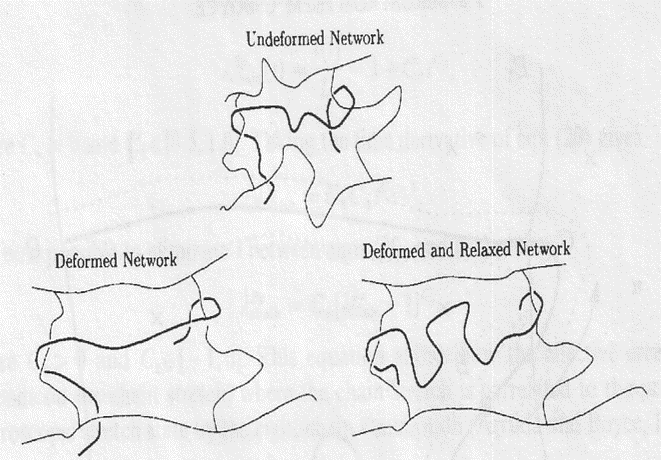
\includegraphics[width=0.7\linewidth]{volny-retezec}
	\caption{Volný řetězec v~síti}
	\label{fig:volny-retezec}
\end{figure}

Přestože se volné řetězce v~makromolekulární síti elastomerů nevyskytují, existují tam téměř volné konce řetězců, které se chovají podobně.
Po deformaci se napnou a~postupně se vracejí do více zvlněného stavu s~vyšší entropií.
\begin{figure}[H]
	\centering
	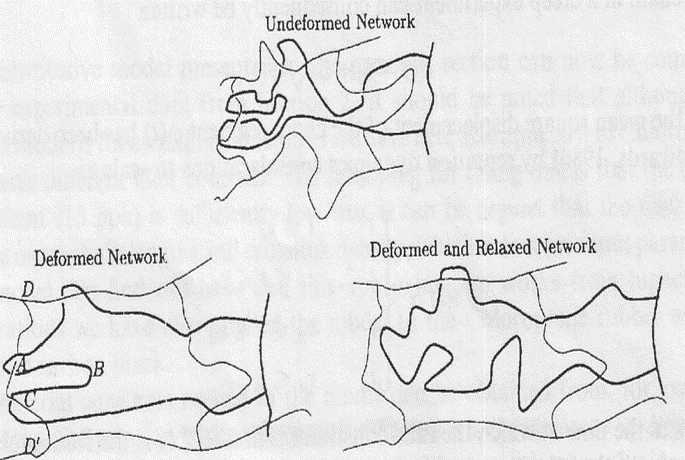
\includegraphics[width=0.7\linewidth]{temer-volne-konce-retezcu}
	\caption{Téměř volné konce řetězců}
	\label{fig:temer-volne-konce-retezcu}
\end{figure}

\subsubsection{Rovnice modelu Bergstrőm-Boyce}
Pro část~A podle reologického schématu se používá popis Arruda-Boyce, viz rov. (\ref{eq:deformacni-prace-izotermickeho-deje})
\begin{equation}
	W^A = G^A \lambda_L^A \left\{ \lambda_\text{chain} \beta^A - \lambda_L^A \ln\left[ \frac{\sinh\left(\beta^A\right)}{\beta^A} \right] \right\}
\end{equation}

Pro popis části~B se po dekompozici deformačního gradientu na elastickou a~viskózní část použije pro elastickou část~B analogická rovnice jako pro~A
\begin{equation}
	W_\text{el}^B = G^B \lambda_L^B \left\{ \lambda_\text{chain}^\text{el} \beta^B - \lambda_L^B \ln\left[ \frac{\sinh\left(\beta^B\right)}{\beta^B} \right] \right\},
\end{equation}
zatímco viskózní část je popsána následujícím vztahem mezi napětím a~rychlostí deformace
\begin{equation}
	\dot{\gamma} = \gamma_0 \left( \varepsilon_\text{chain}^\text{vis} \right)^C \left( \frac{\tau}{\tau_\text{base}} \right)^m,
\end{equation}
který lze upravit do tvaru
\begin{equation}
	\dot{\gamma} = \frac{\gamma_0}{\tau_\text{base}^m} \left( \lambda_\text{chain}^\text{vis} - 1 + \delta \right)^C \tau^m.
\end{equation}

ANSYS zde využívá ještě rovnici
\begin{equation}
	\lambda_L = \sqrt{N}.
\end{equation}

\subsubsection{Konstanty modelu Bergstrőm-Boyce v~ANSYSu}
Dohromady je ve všech třech částech modelu (reologického schématu) těchto 7 materiálových parametrů (značení podle ANSYSu):
\begin{figure}[H]\label{tab:konstanty-bergstrom-boyce}
	\centering
	\begin{tabular}{ll}\toprule
		Počáteční smykový modul části A & $G_A$ ('C1')\\
		Počet článků řetězce části A & $N_A$ ('C2')\\
		Počáteční smykový modul části B & $G_B$ ('C3')\\
		Počet článků řetězce části B & $N_B$ ('C4')\\
		Creepový parametr & $\tfrac{\gamma_0}{\tau_\text{base}^m}$ ('C5')\\
		Exponent creepové deformace & $C$ ('C6')\\
		Exponent efektivního napětí & $m$ ('C7')\\
	\bottomrule\end{tabular}
\end{figure}

$\delta$ ve vztahu pro viskózní část je matematická konstanta o~malé hodnotě (typicky $\delta \leq \num{0.01}$), která odstraňuje singularitu napětí pro nulové deformace.

\begin{figure}[H]
	\centering
	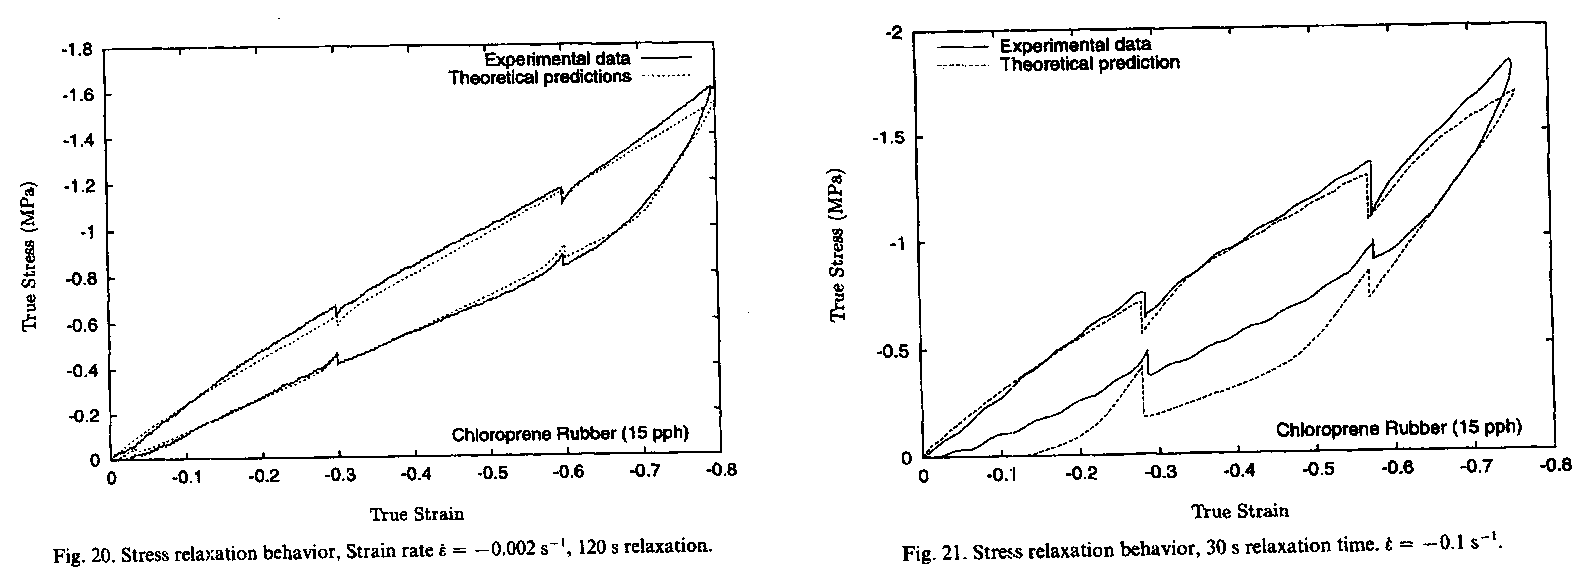
\includegraphics[width=0.9\linewidth]{aproximace-bergstrom-boyce}
	\caption{Aproximace jednoosé tlakové zkoušky s~relaxací během zatěžování i~odlehčování při různých rychlostech deformace}
	\label{fig:aproximace-bergstrom-boyce}
\end{figure}
